%presentation
\documentclass{beamer}

%impressions
%\documentclass[handout]{beamer}
%\usepackage{pgfpages}
%\pgfpagesuselayout{2 on 1}[a4paper,border shrink=5mm]
%\setbeameroption{notes on second screen}
%\pgfpagelayout{2 on 1}[a4paper, border, shrink=5mm]
% vue sur http://wwwtaketorg/spip/articlephp3?id_article=30...
%\usepackage[T1]{fontenc}
\usepackage[frenchb]{babel}
\usepackage[utf8x]{inputenc} % Pour pouvoir taper les accents sans faire de combinaison
%\usepackage{arev}
%\usepackage{aeguill}
%mode code
\usepackage{listings}

%mode verbatim
\usepackage{moreverb}

%\usepackage[darktab]{beamerthemesidebar}
%\leftsidebar
%\usetheme{Hannover}
%\usetheme{Warsaw}
%\usetheme{PaloAlto}
\usetheme{JuanLesPins}
%\usetheme{Antibes}
%\usetheme{Shingara}
%\usetheme{Berlin}
%\usetheme{Oxygen}
\usepackage{thumbpdf}
\usepackage{wasysym}
\usepackage{ucs}
\usepackage{pgfarrows,pgfnodes,pgfautomata,pgfheaps,pgfshade}
\usepackage{verbatim}
\usepackage{color}

\AtBeginSection[]
{
  \begin{frame}<beamer>
    \tableofcontents[currentsection,currentsubsection]
  \end{frame}
}


\title{Cucumber, le texte qui teste}
\author{Cyril Mougel}
\date{2 Octobre 2009}

\logo{
\includegraphics[width=30mm]{cucumber.png}}

\lstset{ 
  breaklines=true
    , language=ruby
    , numbers=left
    , tabsize=2
    , basicstyle=\small\ttfamily
    , keywordstyle=\color{blue}
    , commentstyle=\color{green}
    , stringstyle=\color{red}
    , identifierstyle=\ttfamily
    , columns=fixed
    , showstringspaces=false
}

\begin{document}

\begin{frame}
    \titlepage
\end{frame}

\Large{}

\section{Les tests}

\begin{frame}
  \frametitle{Pourquoi faire des tests ?}
  \begin{itemize}
    \item Etre sûr que ça marche
    \item Valider ce que le client veut 
    \item Eviter les r\'egressions
  \end{itemize}
\end{frame}

\begin{frame}
  \frametitle{Pourquoi automatiser ses tests ?}
  \begin{itemize}
    \item Ne pas perdre son temps à faire toujours les mêmes clics
    \item Temps de test plus court
  \end{itemize}
\end{frame}

\begin{frame}
  \frametitle{Qui d\'efini les tests ?}
  \begin{itemize}
    \item Le client
    \item Le chef de projet
    \item Le d\'eveloppeur
  \end{itemize}
\end{frame}

\begin{frame}
  \frametitle{Quel sont leur langage ?}
  \begin{itemize}
    \item Le client : Le document texte
    \item Le chef de projet : Le document texte
    \item Le d\'eveloppeur : Le code
  \end{itemize}
\end{frame}

\begin{frame}
  \begin{center}
  \Large{}
  Pour aider tout le monde il y a 
  \end{center}
  \begin{center}
    \Huge{}
    Cucumber
  \end{center}
\end{frame}

\section{Cucumber c'est quoi ?}

\begin{frame}
	\frametitle{Cucumber c'est quoi ?}
	\begin{itemize}
    \item Test d'intégration
    \item BDD
    \item Héritier des Stories de Rspec
	\end{itemize}
\end{frame}

\begin{frame}
  \frametitle{Format des tests}
  \begin{itemize}
    \item Business Readable DSL
    \item Fichier texte
  \end{itemize}
\end{frame}

\begin{frame}
  \frametitle{Un exemple ?}
  \begin{beamerboxesrounded}{login.feature}
    %% TODO: add color in cucumber style
    \lstinputlisting[language=,numbers=none]{login.feature}
  \end{beamerboxesrounded}
\end{frame}

\begin{frame}
  \begin{itemize}
    \item But
    \item Rôle
    \item Resultat
  \end{itemize}
\end{frame}

\begin{frame}
  \begin{itemize}
    \item Context
    \item Action
    \item R\'esultat
  \end{itemize}
\end{frame}

\section{installation}

\begin{frame}
  \frametitle{installation}
  \begin{itemize}
    \item gem install rspec rspec-rails cucumber webrat
    \item ruby script/generate cucumber
  \end{itemize}
\end{frame}

\section{utilisation}

\begin{frame}
  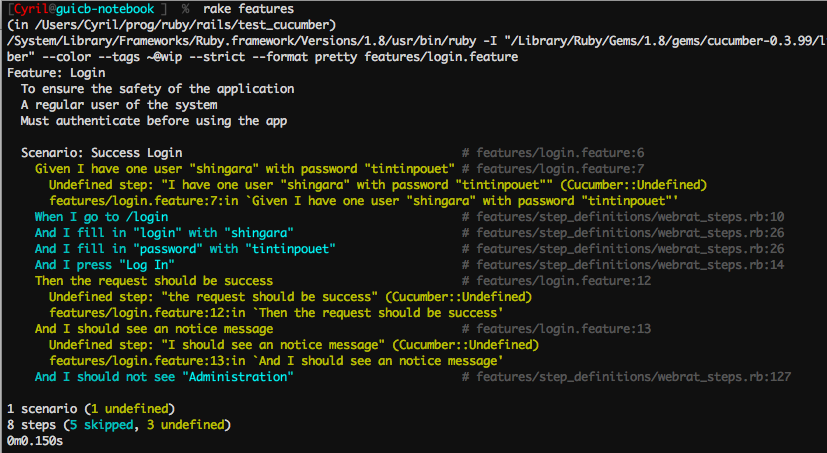
\includegraphics[scale=.4]{features_with_step_undefined}
\end{frame}

\begin{frame}
  \begin{center}
    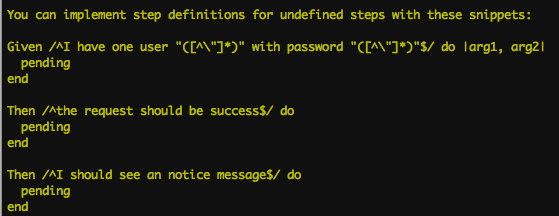
\includegraphics[scale=.5]{step_missing}
  \end{center}
\end{frame}

\begin{frame}
  \begin{tabbing}
    feat\=ures/ \\
    \> login.feature \\
    \> step\=\_definitions/ \\
    \> \> login\_steps.rb \\
  \end{tabbing}
\end{frame}

\begin{frame}
  \frametitle{Given == Setup}
  \begin{beamerboxesrounded}{Given step}
    %% TODO: add color in cucumber style
    \lstinputlisting[numbers=none,basicstyle=\tiny]{given_step.rb}
  \end{beamerboxesrounded}
\end{frame}

\begin{frame}
  \frametitle{When == Modfification}
  \begin{beamerboxesrounded}{When step}
    %% TODO: add color in cucumber style
    \lstinputlisting[numbers=none,basicstyle=\tiny]{when_step.rb}
  \end{beamerboxesrounded}
\end{frame}

\begin{frame}
  \frametitle{Then == R\'esultat}
  \begin{beamerboxesrounded}{Then step}
    %% TODO: add color in cucumber style
    \lstinputlisting[numbers=none,basicstyle=\tiny]{then_step.rb}
  \end{beamerboxesrounded}
\end{frame}

\begin{frame}
    \begin{center}
    \huge{}
    questions ?
    \end{center}
\end{frame}

\end{document}
